% $Header: /home/vedranm/bitbucket/beamer/solutions/generic-talks/generic-ornate-15min-45min.en.tex,v 90e850259b8b 2007/01/28 20:48:30 tantau $

\documentclass{beamer}

% This file is a solution template for:

% - Giving a talk on some subject.
% - The talk is between 15min and 45min long.
% - Style is ornate.



% Copyright 2004 by Till Tantau <tantau@users.sourceforge.net>.
%
% In principle, this file can be redistributed and/or modified under
% the terms of the GNU Public License, version 2.
%
% However, this file is supposed to be a template to be modified
% for your own needs. For this reason, if you use this file as a
% template and not specifically distribute it as part of a another
% package/program, I grant the extra permission to freely copy and
% modify this file as you see fit and even to delete this copyright
% notice. 


\mode<presentation>
{
  \usetheme{Singapore}
  % or ...

  \usecolortheme{beaver}

  \setbeamercovered{transparent}
  % or whatever (possibly just delete it)
}


\usepackage[english]{babel}
% or whatever

\usepackage[utf8]{inputenc}
% or whatever

\usepackage{times}
\usepackage[T1]{fontenc}
% Or whatever. Note that the encoding and the font should match. If T1
% does not look nice, try deleting the line with the fontenc.

\usepackage{comment}
\usepackage{siunitx}
\usepackage{framed}
\usepackage[scaled]{beramono}

\title % (optional, use only with long paper titles)
{A Weather Ontology for Predictive Control in Smart Homes}

%\subtitle
%{Presentation Subtitle} % (optional)

\author[Paul Staroch] % (optional, use only with lots of authors)
{Paul Staroch\\ {\scriptsize paulchen@rueckgr.at}} % TODO smaller mail address
% - Use the \inst{?} command only if the authors have different
%   affiliation.

\institute[Vienna University of Technology] % (optional, but mostly needed)
{
  Arbeitsgruppe Automatisierungssysteme\\
  Institut für Rechnergestützte Automation\\

  \hspace{5em}

  Supervisors:\\
  Ao.Univ.-Prof. Dipl.-Ing. Dr.techn. Wolfgang Kastner\\
  Dipl.-Ing. Mario Kofler

}
% - Use the \inst command only if there are several affiliations.
% - Keep it simple, no one is interested in your street address.

\date % (optional)
{August 27, 2013}

% \subject{Talks}
% This is only inserted into the PDF information catalog. Can be left
% out. 



% If you have a file called "university-logo-filename.xxx", where xxx
% is a graphic format that can be processed by latex or pdflatex,
% resp., then you can add a logo as follows:

\pgfdeclareimage[height=0.5cm]{university-logo}{figures/INF_Logo_typo_grau.pdf}
\pgfdeclareimage[height=0.5cm]{institute-logo}{figures/183-1.pdf}
\logo{\pgfuseimage{university-logo}\hspace{9.4cm}\pgfuseimage{institute-logo}}



% Delete this, if you do not want the table of contents to pop up at
% the beginning of each subsection:
\AtBeginSubsection[]
{
  \begin{frame}<beamer>{Outline}
    \tableofcontents[currentsection,currentsubsection]
  \end{frame}
}


% If you wish to uncover everything in a step-wise fashion, uncomment
% the following command: 

%\beamerdefaultoverlayspecification{<+->}

\DeclareUnicodeCharacter{21D2}{$\Rightarrow$}
\DeclareUnicodeCharacter{2227}{$\wedge$}

\begin{document}

\begin{frame}
  \titlepage
\end{frame}

\begin{frame}{Outline}
  \tableofcontents
  % You might wish to add the option [pausesections]
\end{frame}


% Since this a solution template for a generic talk, very little can
% be said about how it should be structured. However, the talk length
% of between 15min and 45min and the theme suggest that you stick to
% the following rules:  

% - Exactly two or three sections (other than the summary).
% - At *most* three subsections per section.
% - Talk about 30s to 2min per frame. So there should be between about
%   15 and 30 frames, all told.

\section{Introduction}

\begin{frame}{Smart Homes}
	\begin{itemize}
		\item Smart homes are equipped with some kind of intelligence to perform tasks on their own.
		\item Components: Sensors, actuators, communications network, intelligent control.
	\end{itemize}

	Goals:
	\begin{itemize}
		\item Support with routine tasks.
		\item Maintaining or increasing comfort.
		\item Reduction of energy consumption.
	\end{itemize}
\end{frame}

\begin{frame}{Problems of smart homes}
	There are many smart home projects: Mozer's adaptive house, Georgia Tech Aware Home, Gator Tech Smart Home, …

	~

	However, in many cases there are several problems:
	\begin{itemize}
		\item High complexity.
		\item Optimisations and customisations are difficult.
		\item Missing powerfulness and flexibility.
	\end{itemize}

	In many cases, the full potential of smart homes is not exploited.
\end{frame}

\begin{frame}{An ontological approach}
	\begin{center}
		\vspace{-.5cm}
		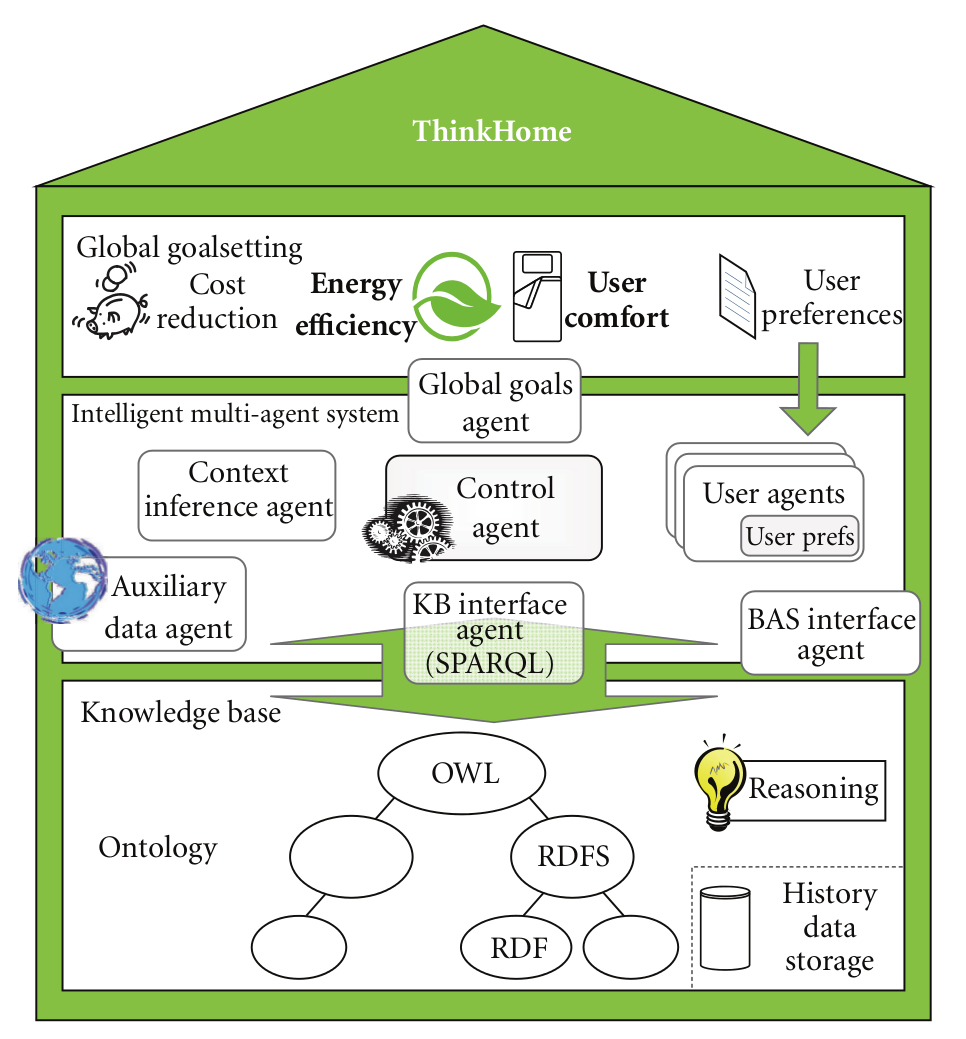
\includegraphics[height=6.5cm]{figures/thinkhome}
	\end{center}
\end{frame}

\begin{frame}{Weather data}
	Processes in and around a dwelling influenced by weather, e.g.:
	\begin{itemize}
		\item Heating, ventilation, and air conditioning (HVAC).
		\item Optimal utilisation of solar and wind power.
		\item Irrigation.
		\item Preparations for severe weather.
	\end{itemize}
\end{frame}

\section{Existing work}

\subsection{Ontologies}

\begin{frame}{Weather ontologies}
	Several ontologies cover weather data:
	\begin{itemize}
		\item Semantic Sensor Web
		\item SSN Ontology
		\item SWEET
		\item NNEW
		\item …
	\end{itemize}

	Unfortunately, none of them was found to be suitable for smart homes.
\end{frame}

\begin{comment}
\begin{frame}{Basic WGS84 (lat/lon) Vocabulary}
	\begin{center}
		\includegraphics[width=.9\textwidth]{figures/dia/wgs84_example}
	\end{center}
\end{frame}

\begin{frame}{OWL-Time (1)}
	\begin{center}
		\includegraphics[width=.9\textwidth]{figures/dia/owl_time_example1}
	\end{center}
\end{frame}

\begin{frame}{OWL-Time (2)}
	\begin{center}
		\includegraphics[width=.6\textwidth]{figures/dia/owl_time_example2}
	\end{center}
\end{frame}

\begin{frame}{Units of Measurement (1)}
	\begin{center}
		Without units:

		~

		\includegraphics[width=.4\textwidth]{figures/dia/nounits_example}
	\end{center}
\end{frame}

\begin{frame}{Units of Measurement (2)}
	\begin{center}
		Measurement Units Ontology:

		~

		\includegraphics[width=.7\textwidth]{figures/dia/muo_example}
	\end{center}
\end{frame}

\begin{frame}{Units of Measurement (3)}
	\begin{center}
		Ontology of Units of Measure and Related Concepts:

		~

		\includegraphics[width=.7\textwidth]{figures/dia/om_example}
	\end{center}
\end{frame}
\end{comment}

\begin{frame}{Related ontologies}
	\begin{itemize}
		\item Location: Basic WGS84 (lat/lon) Vocabulary
		\item Date and time: OWL-Time
		\item Units of Measurement:
			\begin{itemize}
				\item Measurement Units Ontology
				\item Ontology of Units of Measure and Related Concepts
				\item …
			\end{itemize}
	\end{itemize}
\end{frame}

\subsection{Weather data}

\begin{frame}{Sensors and services}
	SmartHomeWeather retrieves data from local weather sensors and Internet weather services.

	\begin{itemize}
		\item Arbitrary number of sources possible.
		\item Assignment of priority values to weather data.
		\item Current data from sensors and services.
		\item Forecast data from services.
		\item Time range for forecasts: 24 hours.
	\end{itemize}
\end{frame}

\begin{frame}{Weather sensors}
	Sensors are commonly accessed via fieldbus systems (KNX, LonWorks, BACnet, …).
	A variety of sensors is available:
	\begin{itemize}
		\item Barometer
		\item Photometer
		\item Hygrometer
		\item Rain gauge
		\item Pyranometer
		\item Thermometer
		\item Wind wane, anemometer
	\end{itemize}
\end{frame}

\begin{frame}{Weather services}
	\begin{itemize}
		\item Weather services evaluated: DWD, Google Weather Feed, METAR, NWS, Weather.com, Weather Underground, World Weather Online, Yahoo! Weather, yr.no.
		\item Criteria for evaluation: Coverage area, data format, data access, access restrictions, terms of use, documentation, stability, weather elements, time frame, weather updates.
		\item Conclusion: Reference implementation using yr.no
	\end{itemize}
\end{frame}

\begin{frame}{Weather elements}
	Weather elements currently used in SmartHomeWeather:
	\begin{itemize}
		\item Temperature
		\item Relative humidity
		\item Dew point
		\item Cloud coverage
		\item Precipitation
		\item Wind
		\item Atmospheric pressure
		\item Solar radiation
		\item Position of the sun
		\item Weather condition
	\end{itemize}
\end{frame}

\subsection{Ontology design methodologies}

\begin{frame}{Methodologies}
	\begin{itemize}
		\item Ontology 101
		\item Uschold and King
		\item TOronto Visual Enterprise
		\item UPON
		\item METHONTOLOGY
	\end{itemize}
\end{frame}

\begin{frame}{METHONTOLOGY}
	\begin{center}
		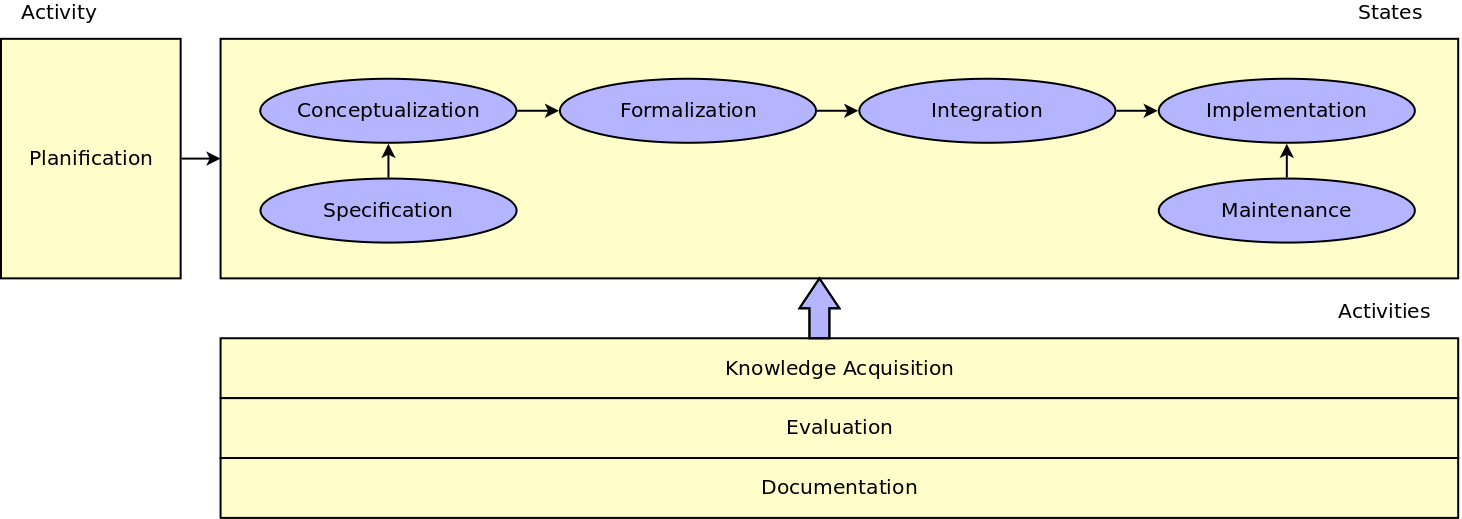
\includegraphics[width=\textwidth]{figures/dia/ontology_lifecycle}
	\end{center}
\end{frame}

\section{Results}

\subsection{SmartHomeWeather}

\begin{frame}{Competency questions}
	\begin{itemize}
		\item What will the weather situation be in one hour, in two hours, …, in 24 hours?
		\item What will be the minimum temperature, humidity, … over the next 24 hours? What about maximum values?
		\item Will the weather change? Will the temperature, humidity, … rise or fall?
		\item Does it rain? Will it rain in the next hours? Will it rain today?
		\item Will temperature drop/stay below \SI{0}{\celsius}?
		\item When can we open windows and when do we have to keep them shut?
	\end{itemize}
\end{frame}

\begin{frame}{Overview}
	\begin{center}
		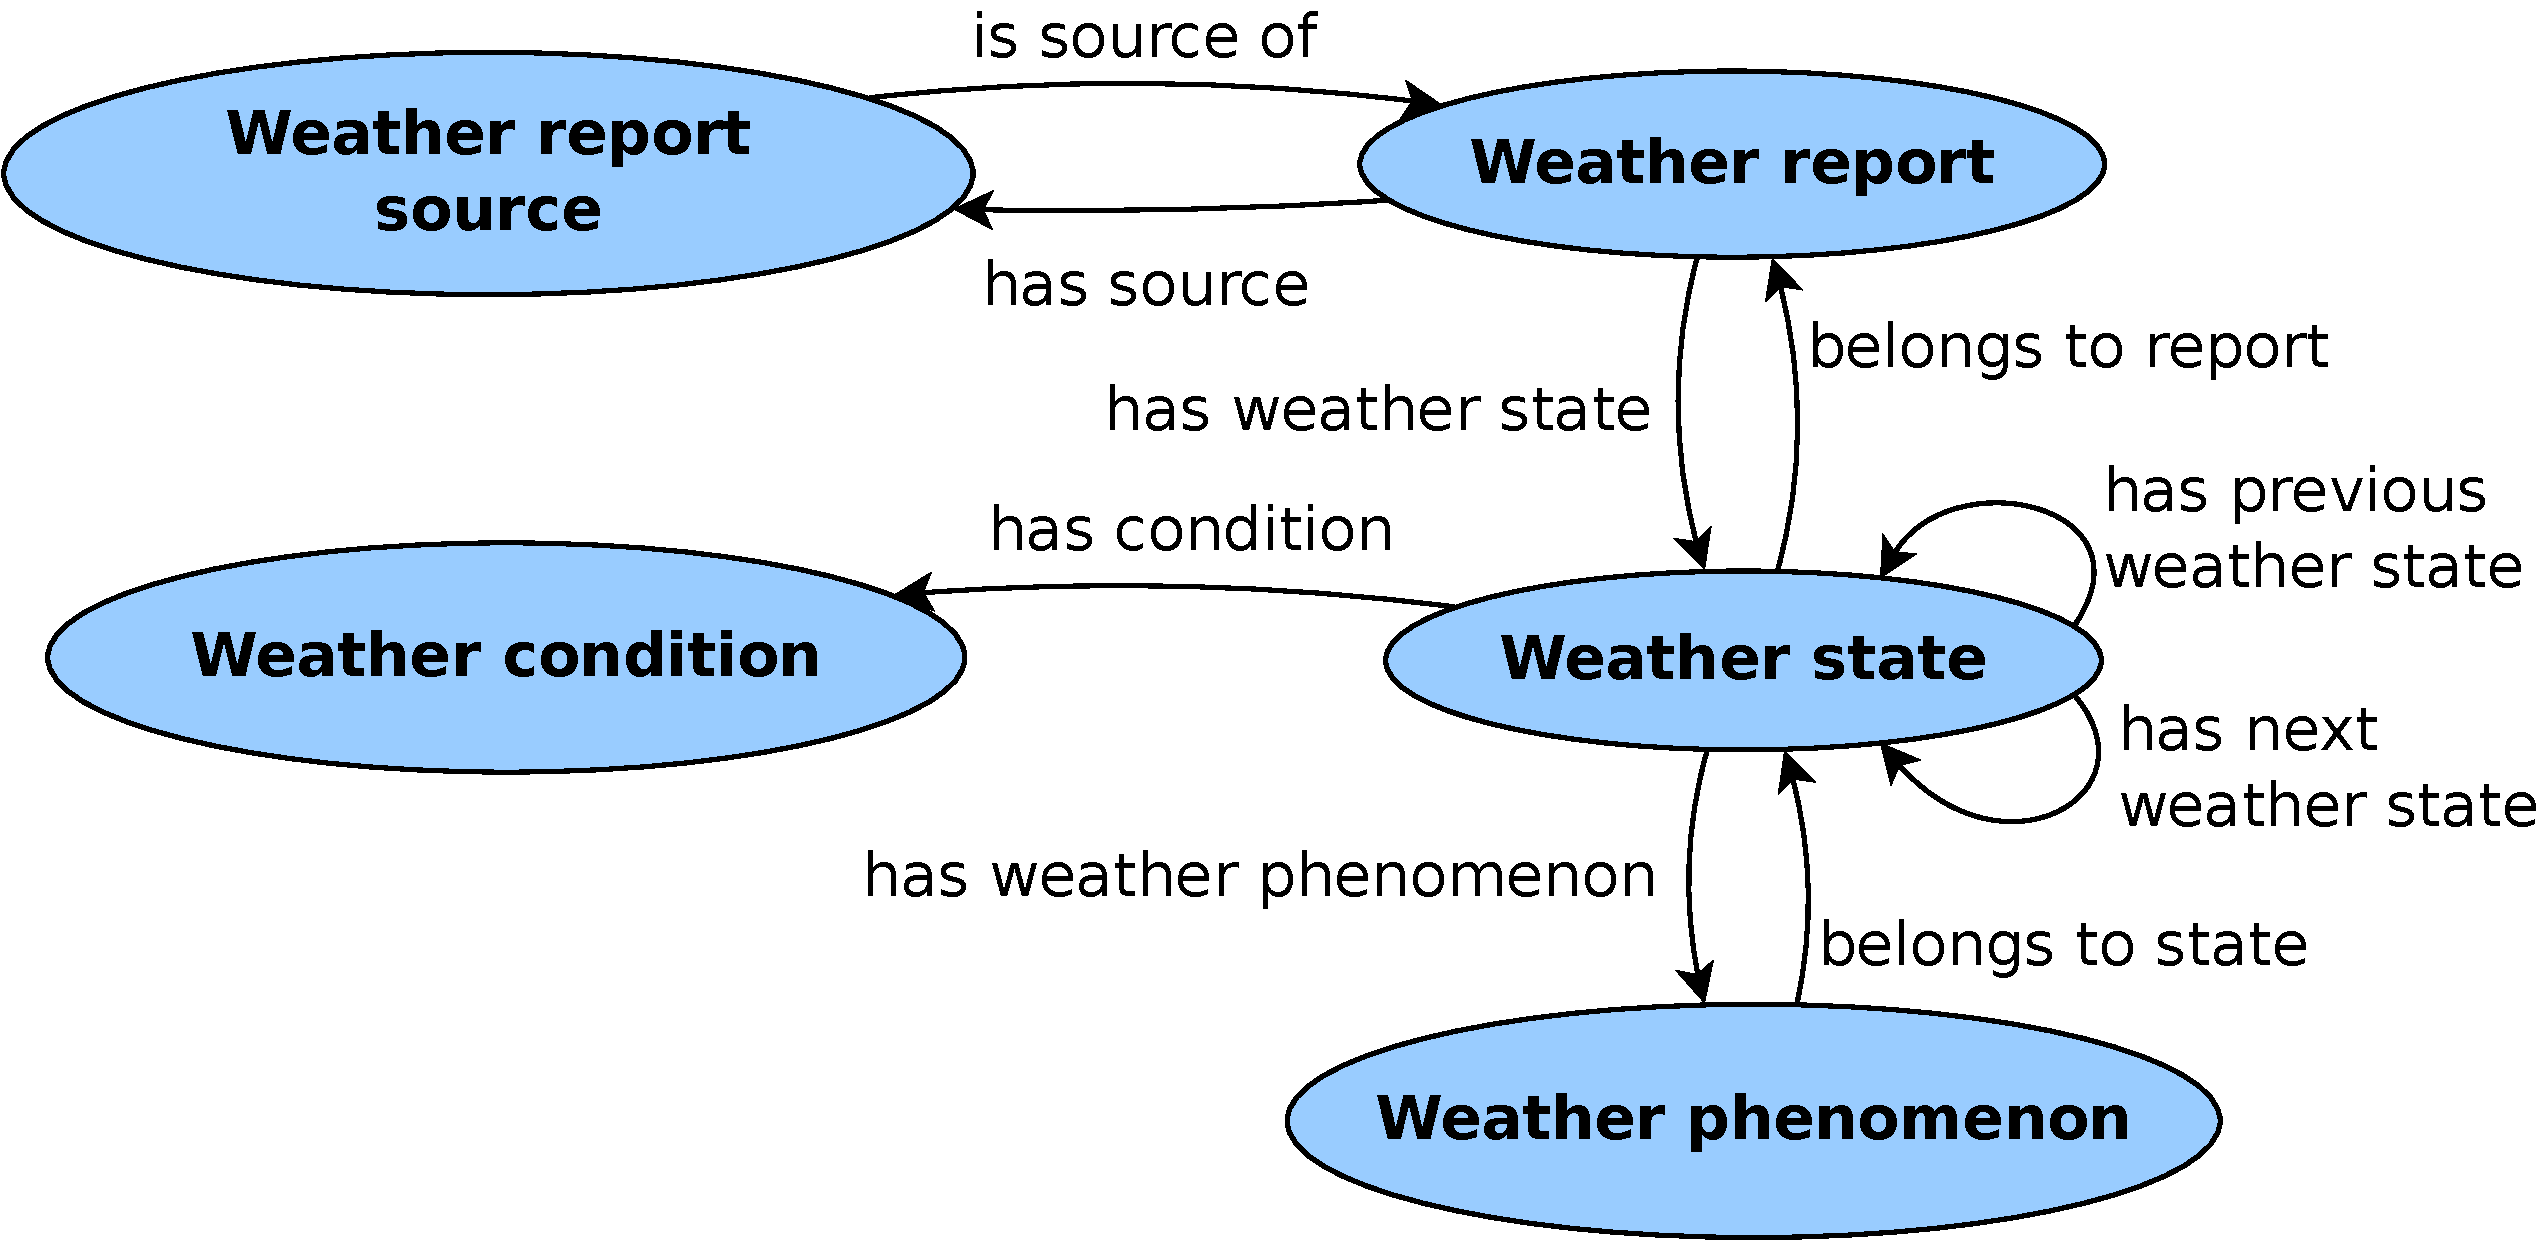
\includegraphics[width=\textwidth]{figures/dia/binary-relations}
	\end{center}
\end{frame}

\begin{frame}{Concept hierarchies: Weather phenomenon}
	\begin{center}
		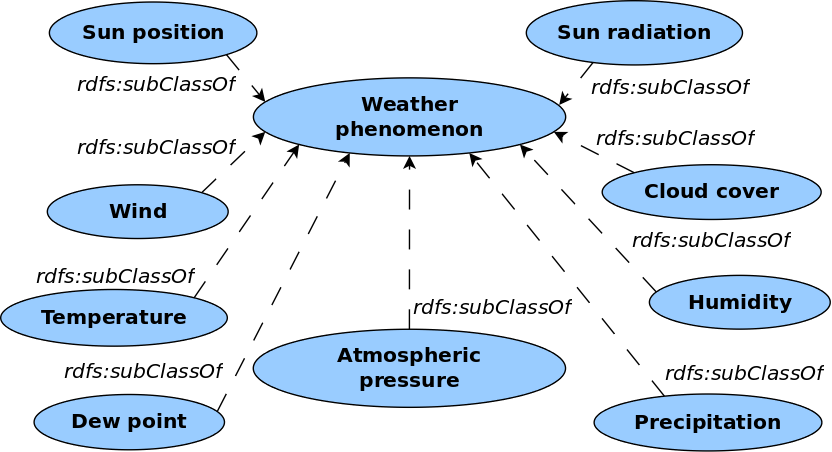
\includegraphics[width=\textwidth]{figures/dia/weather-phenomenon}
	\end{center}
\end{frame}

\begin{frame}{Concept hierarchies: Temperature}
	\begin{center}
		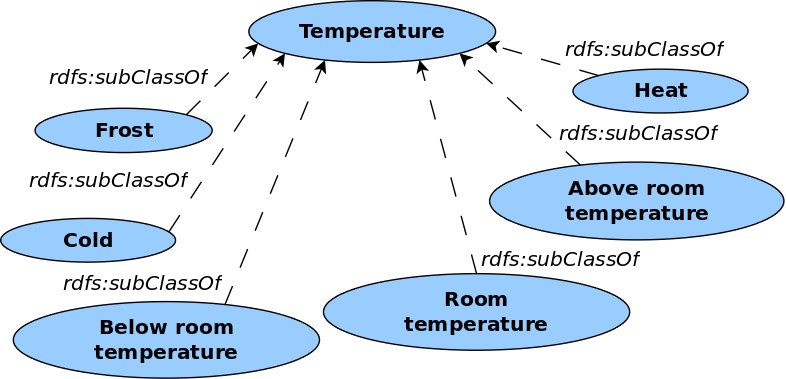
\includegraphics[width=\textwidth]{figures/dia/temperature}
	\end{center}
\end{frame}

\begin{frame}{Concept hierarchies: Weather state}
	\begin{center}
		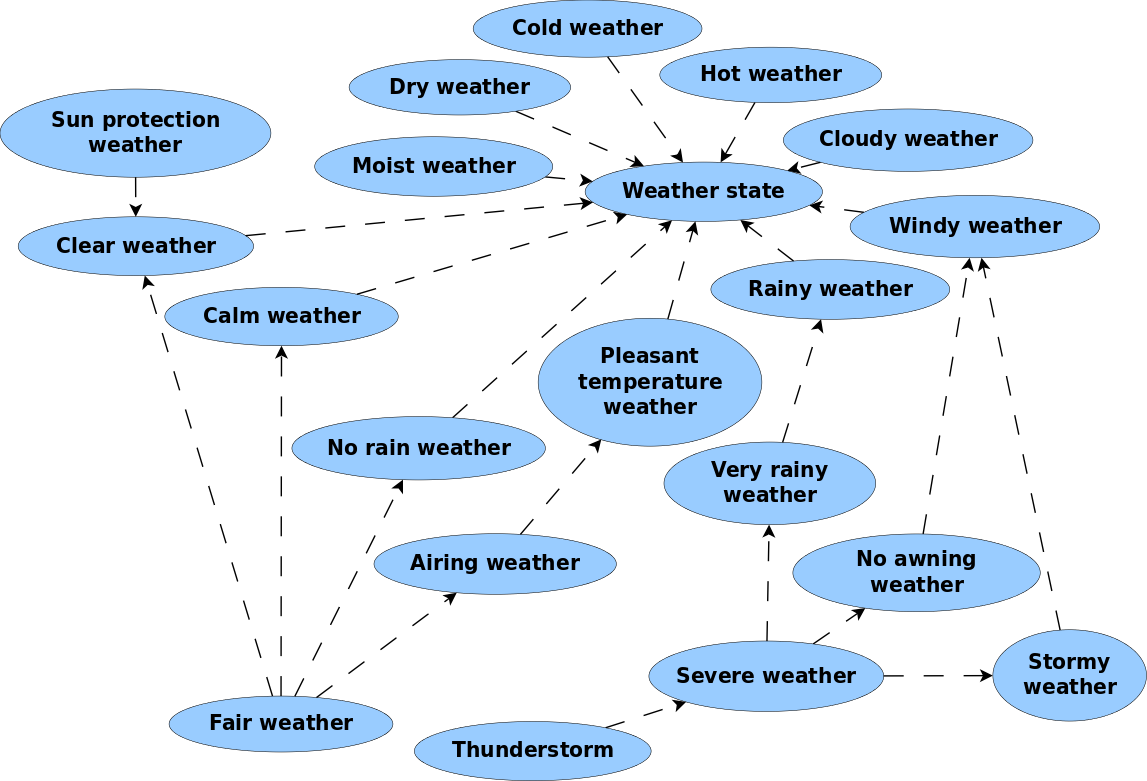
\includegraphics[width=.8\textwidth]{figures/dia/weather-state}
	\end{center}
\end{frame}

\begin{frame}{Concept hierarchies: Weather report}
	\begin{center}
		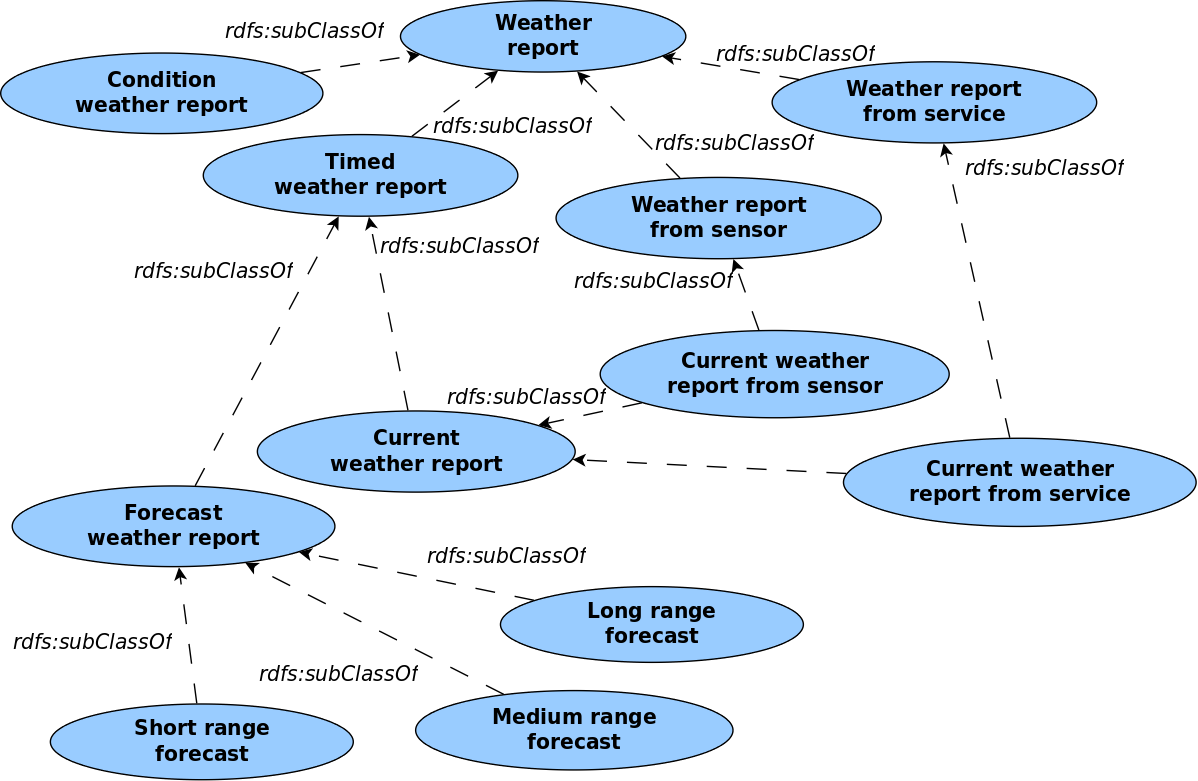
\includegraphics[width=\textwidth]{figures/dia/weather-report}
	\end{center}
\end{frame}

\subsection{Weather Importer}

\begin{frame}{Weather Importer}
	\begin{center}
		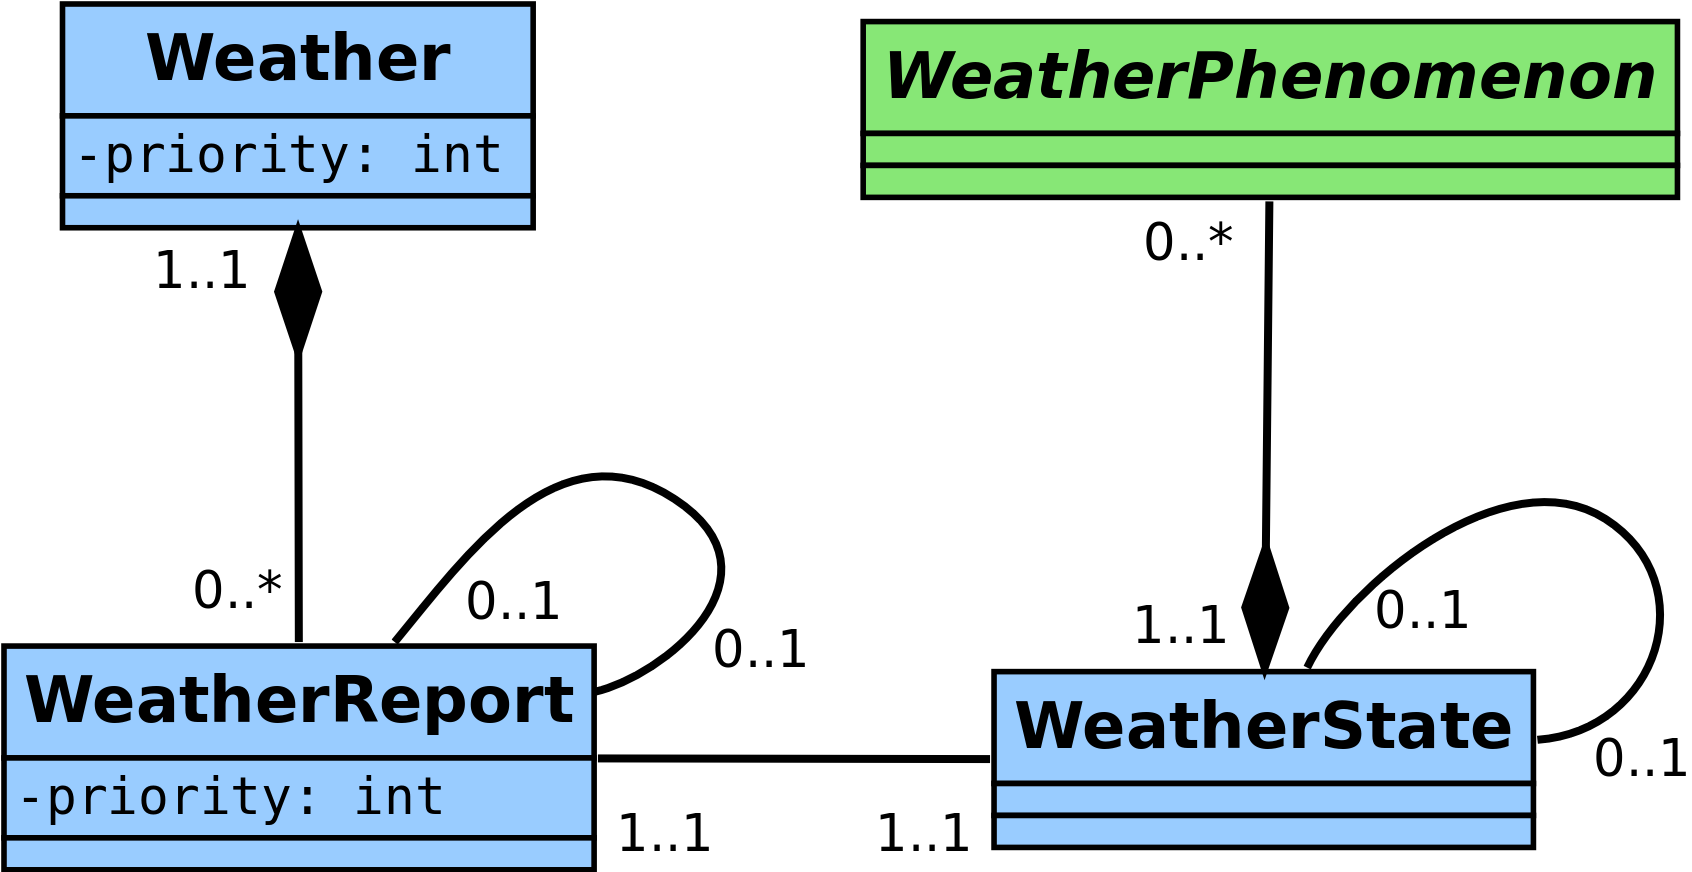
\includegraphics[width=.5\textwidth]{figures/dia/importer-model-simple}
	\end{center}

	\begin{itemize}
		\item Import from sensors and Internet services.
		\item Unit tests for SmartHomeWeather and Weather Importer.
	\end{itemize}
\end{frame}

\begin{frame}[fragile]{SPARQL and SWRL (1)}
	\begin{framed}
		\begin{verbatim}
SELECT ?s
WHERE {
    ?s weather:hasWeatherPhenomenon ?p.
    ?p a weather:Frost.
    ?s weather:belongsToWeatherReport ?r.
    ?r a weather:ShortRangeForecastReport.
}
		\end{verbatim}
	\end{framed}
\end{frame}

\begin{frame}[fragile]{SPARQL and SWRL (2)}
	\begin{framed}
		\begin{verbatim}
hasWeatherPhenomenon(?s1, ?t1) ∧
  hasTemperatureValue(?t1, ?v1) ∧
  numericalValue(?v1, ?m1) ∧
  hasWeatherPhenomenon(?s2, ?t2) ∧
  hasTemperatureValue(?t2, ?v2) ∧
  numericalValue(?v2, ?m2) ∧
  greaterThan(?m2, ?m1) ∧
  hasLaterWeatherState(?s1, ?s2)
   ⇒ increasingTemperature(?s1, ?s2)
		\end{verbatim}
	\end{framed}
\end{frame}

\subsection{Conclusion}

\begin{frame}{Future work}
\end{frame}

\begin{frame}{The end}
\end{frame}

\end{document}


